\section{Analysis and Failure Modes}
\label{sec:analysis}

\subsection{Where tuning helps most}

The tuned model's gains are not evenly distributed across the validation set. Figure~\ref{fig:adaptation-summary} already shows the broad pattern: adaptation helps most when the answer is recoverable from OCR tokens, especially after normalization. Compared with the strongest zero-shot finalist, the tuned model improves validation accuracy by 4.98 points for direct OCR matches and by 7.46 points for answers that become recoverable only after normalization. The gain is still positive when the answer is absent from OCR entirely (+5.57 points), but it is smaller than the gain on normalized OCR-grounded cases. This is a useful result for interpretation. Fine-tuning is not merely making the model more generally capable; it appears to improve how the model uses text that is already present but noisy, fragmented, or only approximately aligned with the canonical answer string.

The OCR-count buckets tell the same story at a different level of granularity. Validation accuracy on OCR-free cases is unchanged at 66.09\%, whereas OCR-rich cases improve substantially: +4.52 points for 1--5 OCR tokens, +5.85 for 6--15, +8.46 for 16--30, and +9.09 for 31+ tokens. In other words, the strongest adaptation gains occur exactly where TextVQA is most text dependent. This makes the final model more convincing as a TextVQA system rather than merely as a stronger short-answer VQA model.

The answer-length analysis also sharpens the interpretation. The tuned model improves one-token answers by 5.85 points, 2--3-token answers by 6.31 points, and 4+-token answers by 7.09 points. Even after tuning, however, long answers remain the hardest category: 76.69\% validation accuracy versus 85.63\% for one-token answers. The gain is therefore real but not saturating. Parameter-efficient tuning helps on harder answer forms, yet does not eliminate the structural difficulty of longer free-form answers.

Question-prefix breakdowns point in the same direction while satisfying a more conventional per-category analysis. Table~\ref{tab:question-prefix} shows that the tuned model improves every validation prefix group with at least 50 examples. The largest gains appear on \texttt{where}, \texttt{which}, \texttt{how}, and the heterogeneous \texttt{other} bucket, whereas \texttt{who} improves more modestly from an already strong zero-shot baseline. This pattern suggests that LoRA is not only correcting a narrow answer-format artifact; it improves several common question forms, with especially large gains where the answer often depends on locating or normalizing visible text.

\begin{table}[t]
    \centering
    \small
    \begin{tabular}{lrrrr}
\toprule
Question prefix & Count & Zero-shot & Tuned & Gain\\
\midrule
what & 3911 & 77.76 & \textbf{83.38} & 5.63\\
who & 236 & 83.05 & \textbf{85.59} & 2.54\\
how & 184 & 75.00 & \textbf{83.70} & 8.70\\
other & 176 & 76.14 & \textbf{88.64} & 12.50\\
is & 162 & 92.59 & \textbf{99.38} & 6.79\\
which & 100 & 83.00 & \textbf{92.00} & 9.00\\
where & 89 & 79.78 & \textbf{93.26} & \textbf{13.48}\\
\bottomrule
\end{tabular}

    \caption{Official validation accuracy by question prefix for prefix groups with at least 50 examples. Bold entries mark the better system within each prefix group and the largest observed gain.}
    \label{tab:question-prefix}
\end{table}

\subsection{Qualitative evidence}

\begin{figure*}[t]
    \centering
    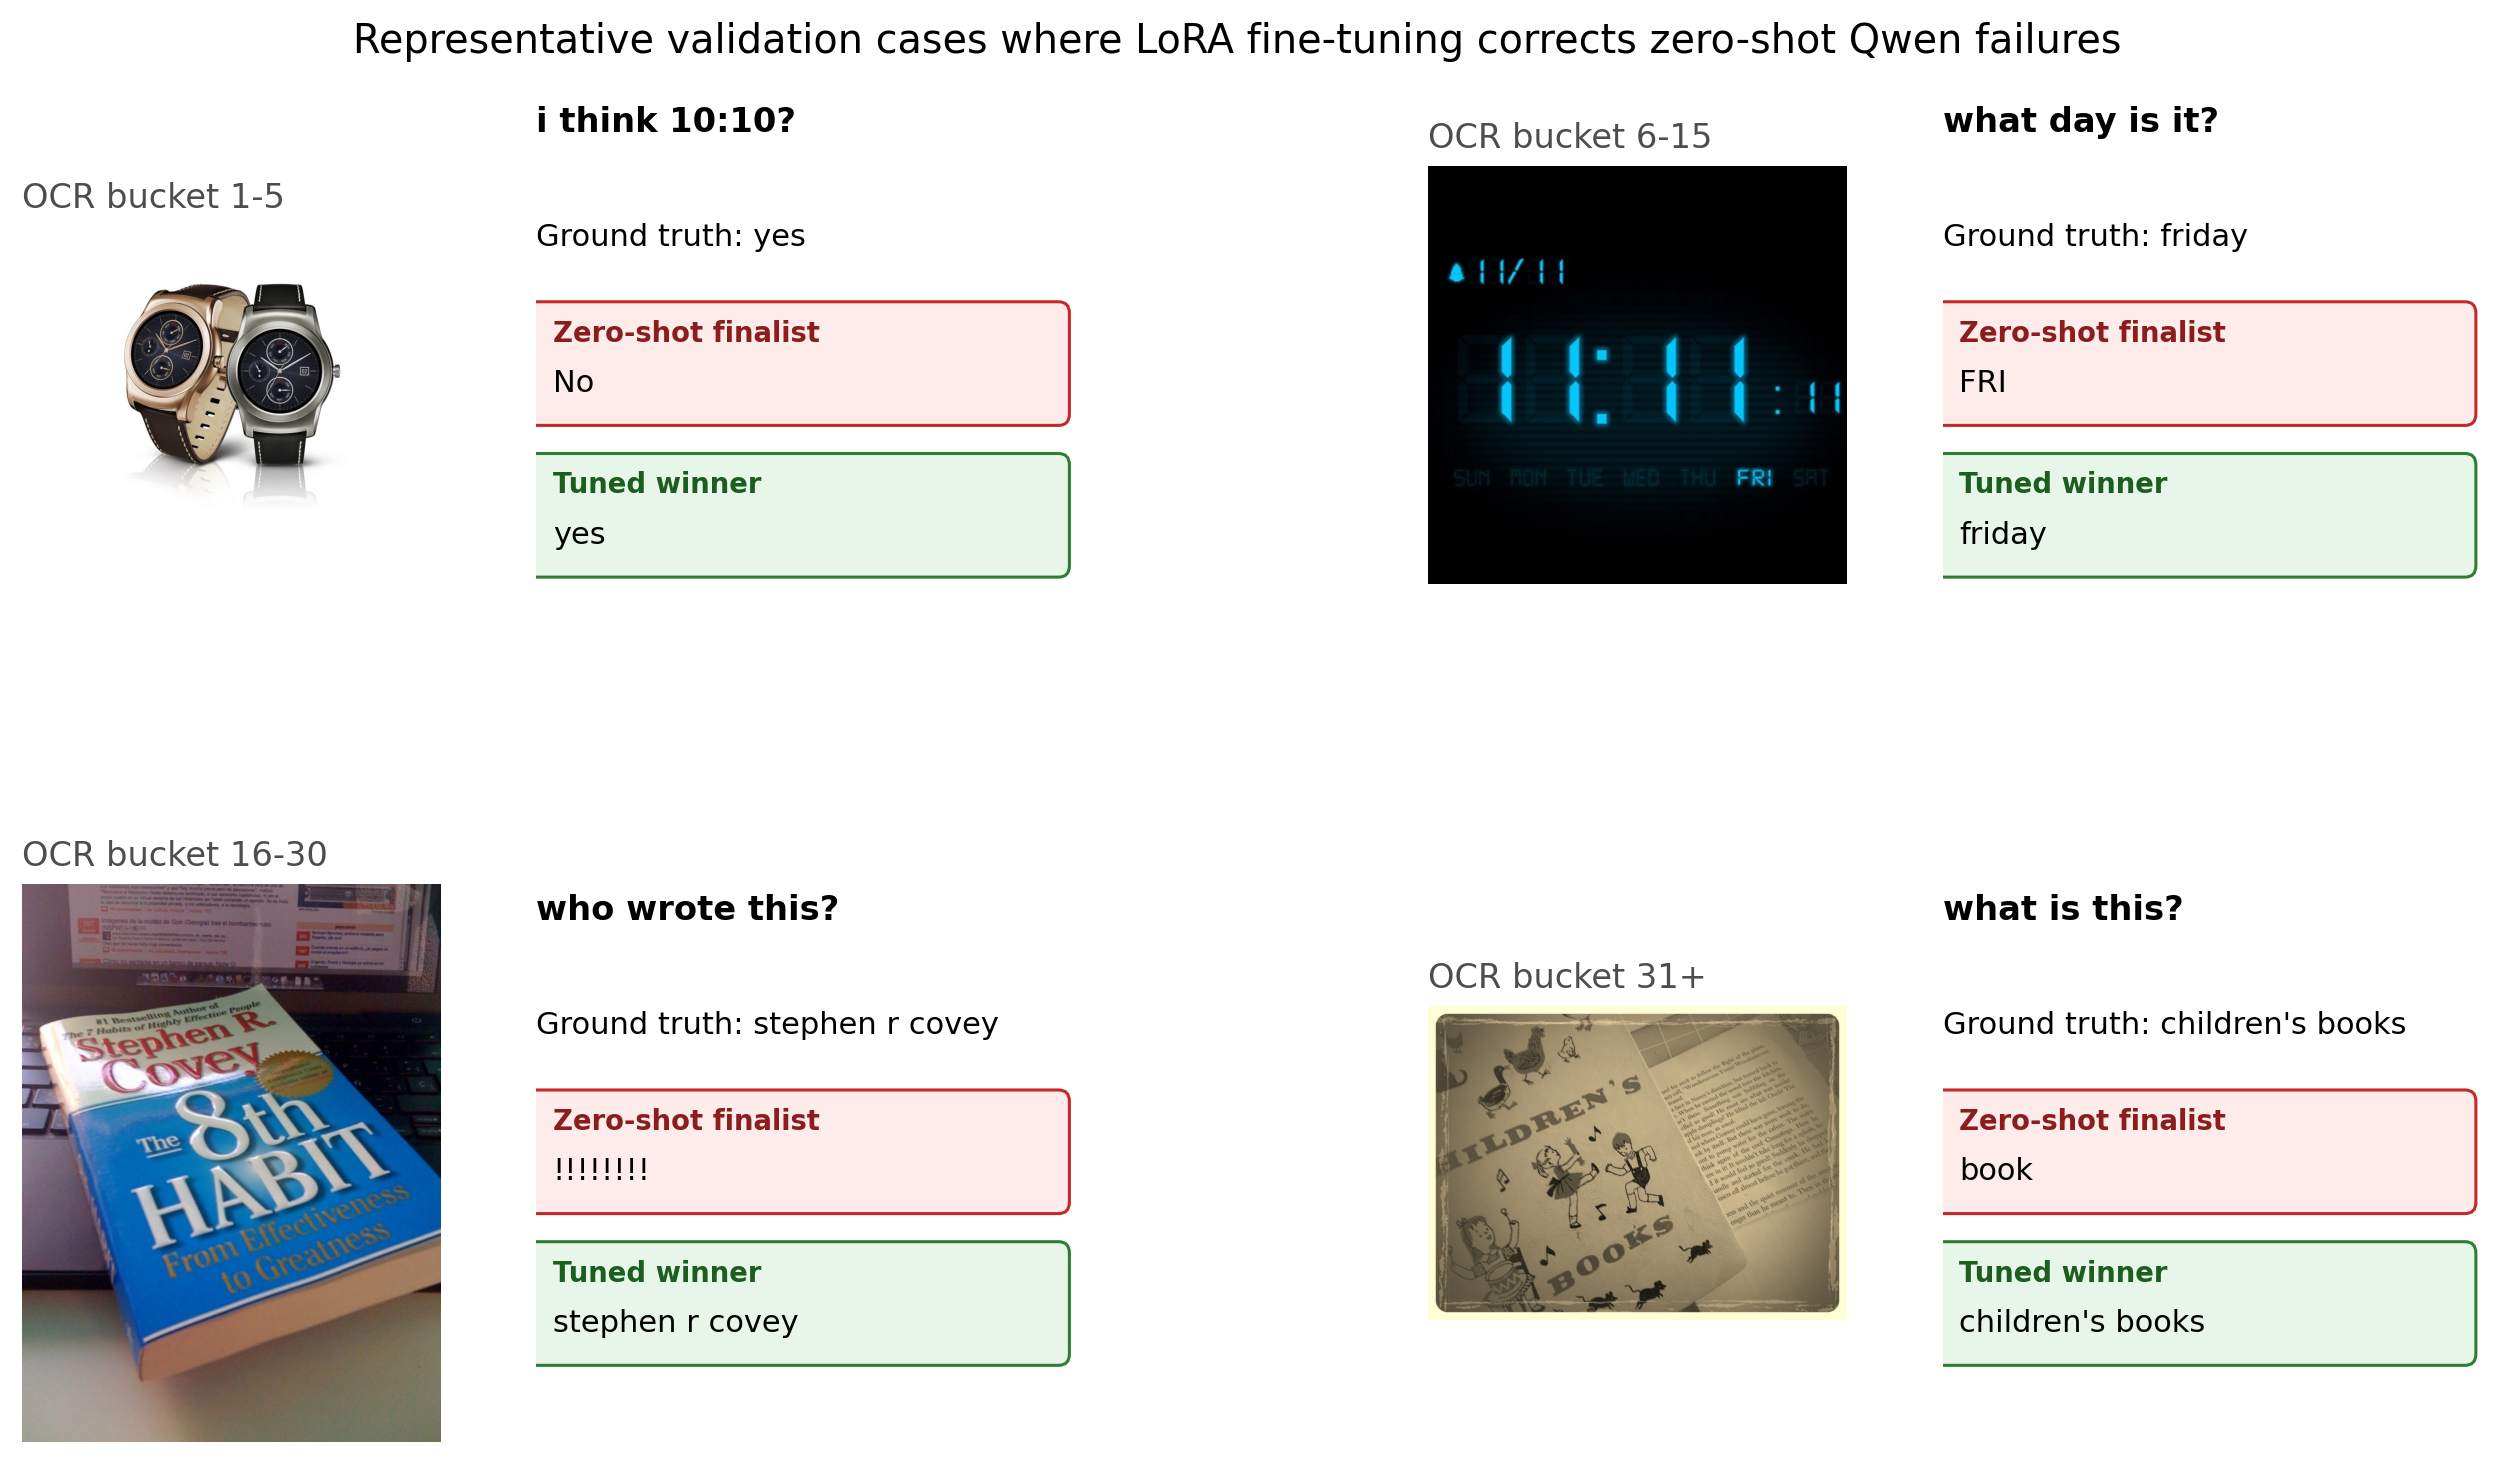
\includegraphics[width=\textwidth]{figures/qualitative_examples.png}
    \caption{Representative validation cases where LoRA fine-tuning corrects failures made by the zero-shot Qwen finalist. The selected examples span OCR buckets from sparse text to dense text and illustrate three recurring recovery patterns: stricter answer-length control (top left), more faithful OCR grounding (top right), and better normalization or denoising of noisy book-cover text (bottom row).}
    \label{fig:qualitative}
\end{figure*}

Figure~\ref{fig:qualitative} makes the qualitative pattern concrete. In the sparse-OCR watch example, the zero-shot finalist over-predicts the visible time string rather than answering the binary question, while the tuned model emits the short categorical answer required by the task. In the digital-clock example, zero-shot Qwen partially reads the day token but returns an abbreviated form that fails exact matching, whereas the tuned model normalizes it to the expected answer. The book-cover examples are even more revealing: the tuned model recovers author and title strings from cluttered or degraded text where the zero-shot model either hallucinates punctuation or collapses the answer to an underspecified noun. These cases are consistent with the bucket analysis above. The fine-tuned system is not simply more verbose or more aggressive; it is more disciplined in turning OCR evidence into task-compatible short answers.

\subsection{Failure modes and limits}

The study also exposes limits that remain after tuning. First, OCR-free questions remain a relative weakness. The tuned model does not improve the zero-shot finalist on the zero-OCR bucket, which suggests that the observed gains are genuinely tied to text-grounded reasoning rather than to a uniform shift in visual question answering quality. Second, despite strong overall improvements, the tuned system is still materially worse on longer answers and on some semantically ambiguous prompts. Third, the OCR ablation follow-up indicates that explicit OCR injection is not the sole driver of post-train gains; once the LoRA adapter is learned, the model appears to internalize part of the text-grounding benefit, but this also makes it harder to isolate exactly which adaptation parameters are compensating for OCR-format differences.

Figure~\ref{fig:failure-examples} shows four official-validation failures that make these limits concrete. The first is a pure visual reading error: both systems misread an analog clock, and the dataset OCR tokens are essentially unhelpful. The second is the opposite failure mode: dataset OCR contains \texttt{HOLLAND}, but the tuned model answers \texttt{italy}, suggesting that visual priors can still override usable text evidence. The third case shows truncation on a long sign answer; the tuned model recovers the beginning of the red-sign offer but not the full phrase required by exact match. The fourth case is a grounding failure in a sports image, where the model locks onto the wrong jersey number despite nearby OCR-like evidence. These examples are not exceptions to the aggregate result; they define the remaining boundary of the tuned system. LoRA improves OCR-grounded answer formation, but it does not fully solve fine-grained time reading, target localization, long-span transcription, or conflicts between visual priors and noisy OCR.

\begin{figure*}[t]
    \centering
    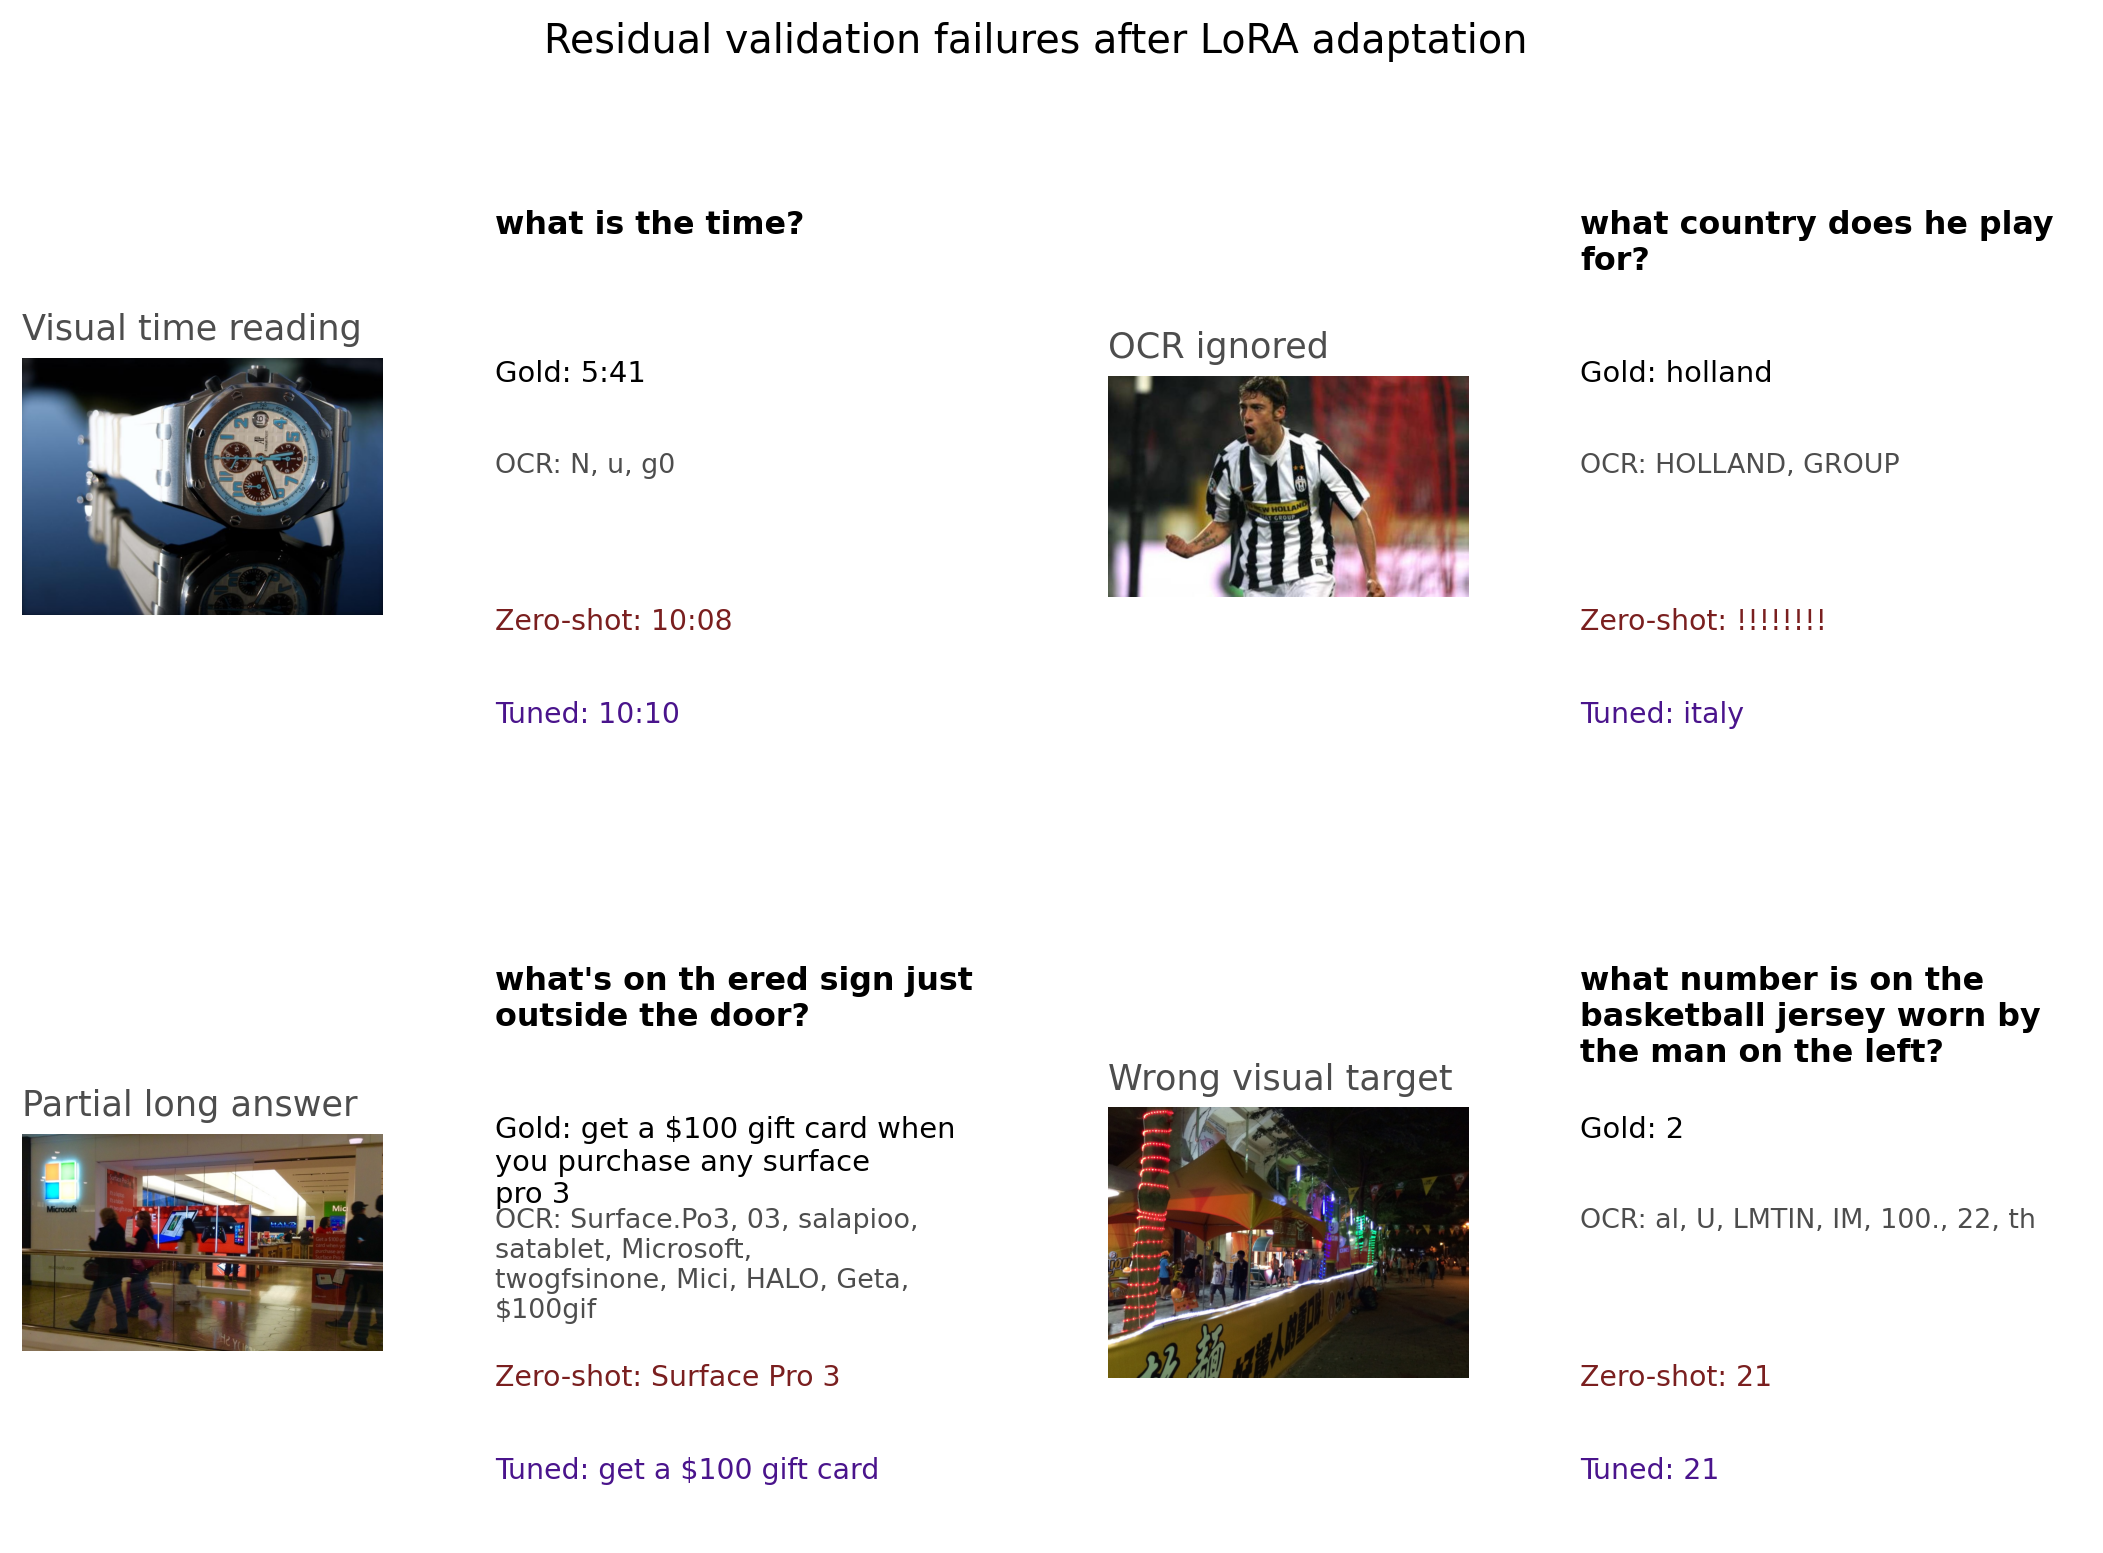
\includegraphics[width=\textwidth]{figures/failure_examples.png}
    \caption{Residual official-validation failures after LoRA adaptation. Each panel reports the question, first human reference answer, dataset OCR snippet, zero-shot Qwen prediction, and tuned-model prediction. The examples show four distinct residual errors: visual time reading without useful OCR, ignoring a correct OCR token, returning only a partial long text answer, and grounding the answer on the wrong visual target.}
    \label{fig:failure-examples}
\end{figure*}

There is also an important methodological limit in the internal-dev split. As Table~\ref{tab:split-audit} reports, internal-dev is question-disjoint but not fully image-disjoint from the LoRA training pool. A post-hoc sensitivity audit partly bounds the issue: for the selected \texttt{all-linear-r16-seed13} adapter, internal-dev accuracy is 88.45\% overall, 88.87\% on image-overlap questions, and 87.39\% on the 571 image-disjoint questions. This confirms that the internal-dev score is slightly higher on overlapping images, so we do not treat internal-dev as final held-out evidence. It also shows that the selected adapter remains strong on the image-disjoint subset, and the final claim is ultimately based on the official validation result rather than on internal-dev alone.

Although the final paper includes API-backed LLM-as-a-Judge scores across the reported experiment tables, we do not use that score as a global replacement for benchmark-native exact match. The judge is most useful as a secondary semantic lens: it tells us whether leaderboard differences survive a more tolerant reading of short answers and whether exact-match gaps are mostly semantic or mostly formatting driven. That is worthwhile additional evidence, but it does not eliminate the need for deterministic, reproducible benchmark metrics across the rest of the study.

Finally, the adaptation story is intentionally narrow. We tune only the selected Qwen backbone and only with LoRA. That decision is scientifically coherent with the funnel design and with the available compute budget, but it leaves open at least two follow-up questions: whether the same winner-conditioned protocol would select a different adaptation family on a larger backbone, and whether a richer parameter-efficient method would preserve the same OCR-grounded gains without increasing instability or cost.
